本システムの機能検証の為に,ユーザーテストを行った.
本章では,ユーザーテストの結果を報告し,考察する.

\section{機器監視機能のテスト}
必要となる機能が実装されていることを確認するため,検証を行った。

\subsection{シナリオ}
ユーザーテストは,1台のIoT機器で成り立っているIoTサービスを想定し行った.
IoT機器には,RaspberryPiを使用する。
図\ref{fig:device}は使用したRaspberryPi2と,IntelEdisonである。
IntelEdisonは今回は使用していないが,エージェントプログラムは動作するはずである。
%IoT機器の図
\begin{figure}[htbp]
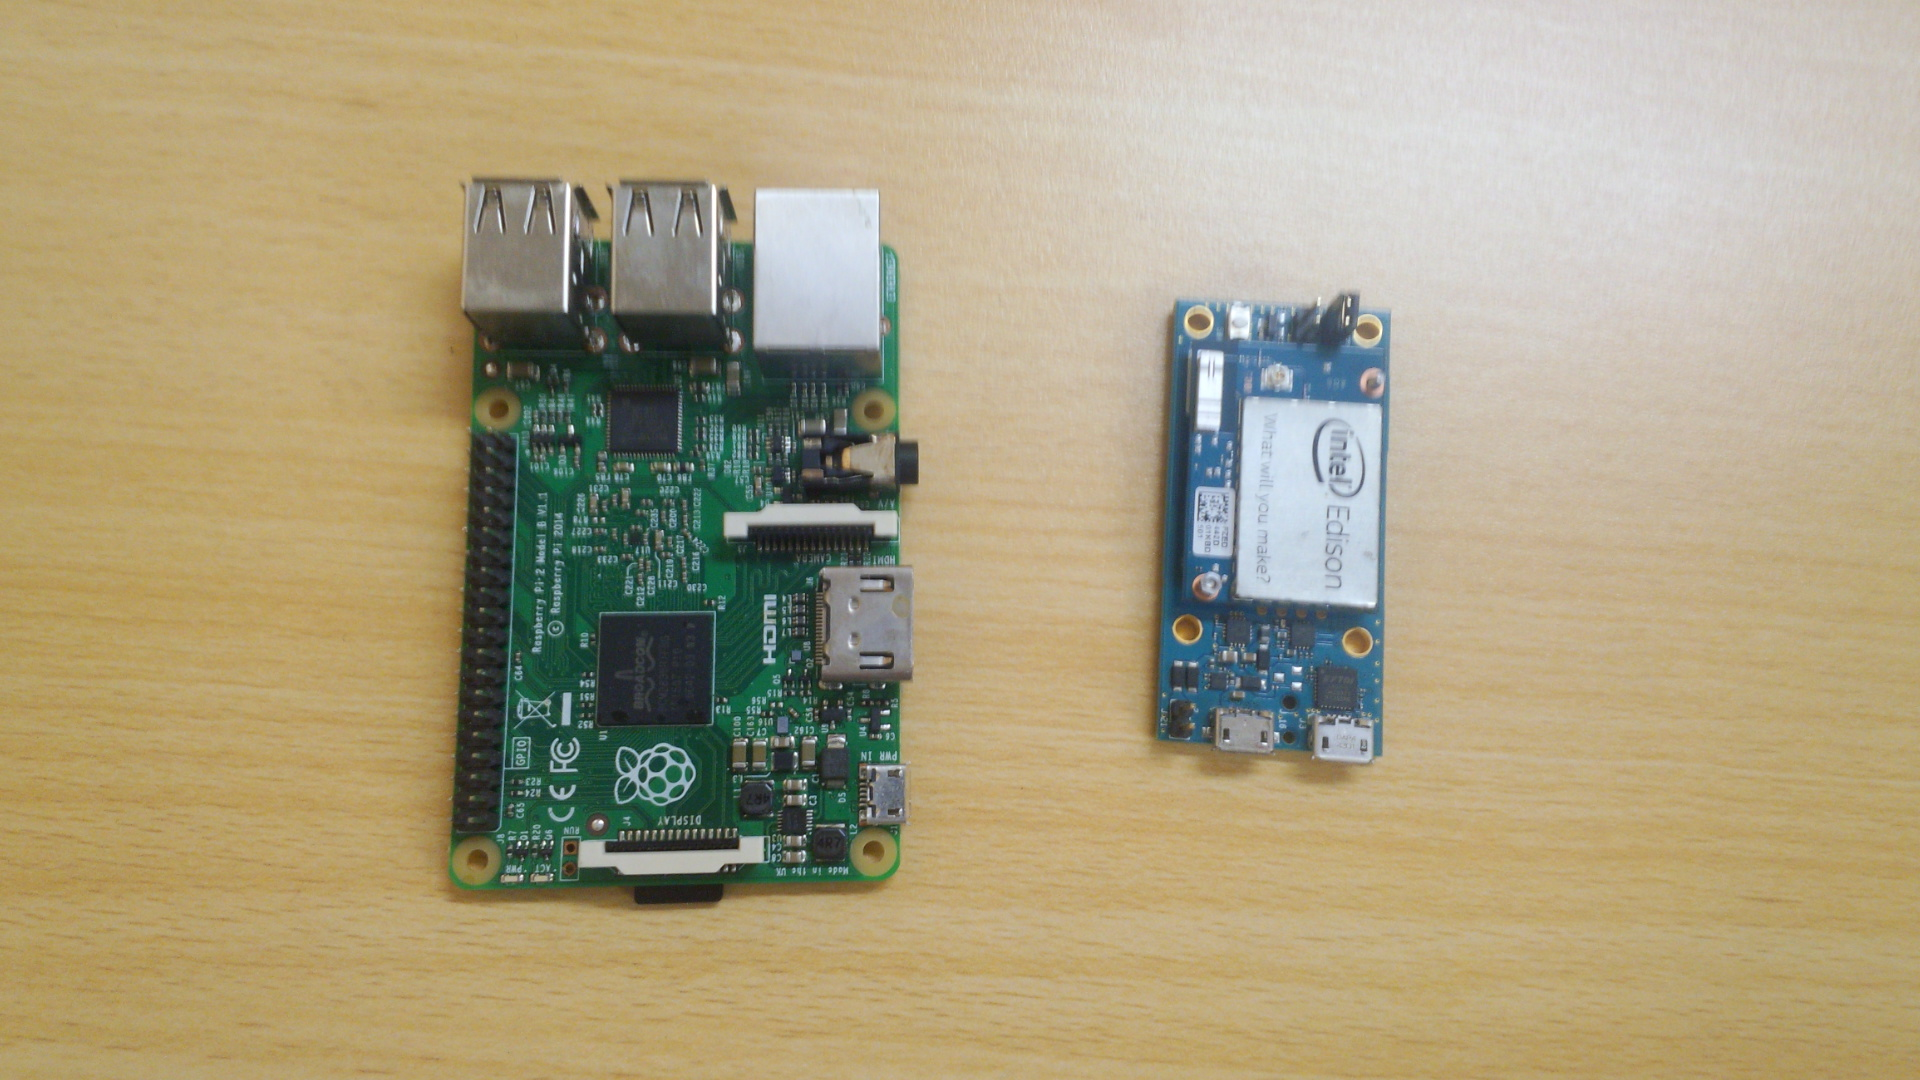
\includegraphics[width=14cm]{images/device.png}
\caption{IoTサービスの構成図}
\label{fig:device}
\end{figure}

RaspberyPi2は無線LANインターフェースを持たないので,バファロー製の無線LANインターフェースを使用した。

期間は2017年1月28日正午から1時間行い,途中何度かIoT機器(RaspberryPi)の電源を抜き,正常に検知することを確認する。
その後,電源が抜けていた期間について,IoT機器の記録を確認する。

\subsection{経過観察}




\section{手順の比較}
従来手法による監視の手間と,本サービスによる監視の手間を比較する.
ここでは,従来の手法として,TelegrafとInfluxdb,Grafanaを用いた機器状態の監視システムを比較対象に挙げる.

順に結果を報告する.
\subsection{機器監視サーバーの構築}
従来の手法では,機器監視をするために,次の様な手間があった.
\begin{enumerate}
\item 機器監視の為にサーバーを用意する
\item 機器監視サーバへInfluxdbをインストールする
\item 機器監視サーバーへGrafanaをインストールする
\item Influxdbに対し,Telegrafとの通信に用いるインターフェースの設定を行う
\item Grafanaに対し,Influxdbと連携するための設定をする.
\end{enumerate}

本サービスを用いる場合,これら準備は不要となる.

\subsection{各IoT機器の状態を可視化する}
従来の手法ではIoT機器の状態を可視化するまでに以下の手順を踏んでいた.
\begin{enumerate}
\item IoT機器にTelegrafをインストールする
\item IoT機器にインストールされたTelegrafの接続先の設定を行う
\item 各IoT機器固有のIDをTelegrafに設定する.
\item Grafanaにログインする.
\item Grafanaへ,現在の状態を表示する為のデータベースクエリを入力する.
\item Grafanaへ,過去の状態を表示するためのデータベースクエリを入力する.
\item 各描画パネルに対し,機器名を設定する.
\end{enumerate}

本サービスでは次の手順を踏む。
\begin{enumerate}
\item 本サービスにログインする
\item 本サービスの機器追加ボタンを押し,機器IDをメモ(コピー)する.
\item 本サービスに対し,機器名と機器詳細を入力する.
\item IoT機器にエージェントプログラムをインストールする.
\item IoT機器にエージェントプログラムを自動で起動するよう設定する.
\end{enumerate}

比較すると,Grafanaへデータベースクエリを入力する作業が,なくなっている.
代わりに,自動起動の為の設定ファイルを設定する手順が増えている.

\section{考察}
ユーザーテストから本システムは,ある程度有効であることが分かったが,以下の点について課題があることが分かった.
\begin{itemize}
\item 機器への設定について\\
	設定ファイルの編集等の手間は削減されたが,エージェントプログラムをIoT機器にインストールするのに手間がかかっていることが分かった.
	従来手法を用いて機器の監視をする際は,自動起動の設定を行う必要はなかったが,本プログラムでは必要としている.
	自動起動の為の設定ファイルを自動生成するか,あるいはエージェントプログラム配布の際,簡単なインストールスクリプト等を一緒に配布することで,大きな手間の削減になると感じでいる.
\item ユーザーインターフェースについて\\
	現在,過去の機器状態の記録については,文字記録として表示しているが,グラフ表示等の方が見やすいと感じた.
	また,期間を指定して閲覧できる機能も必要であることが分かった.
\item エージェントプログラムについて\\
	本サービスで提供しているエージェントプログラムは,その他のパッケージに依存しない単純な構成であるため,移植性が高い.
\end{itemize}


